
\chapter{Planification : à partir de Microsoft Project}

\section{Hiérarchie des tâches}

Le projet est découpé en 6 tâches principales. Les tâches représentent les différentes
étapes techniques par lesquelles nous devrons passer pour développer le projet.

\begin{itemize}
\item préparation des données ;
\item stockage des données ;
\item interface avec le reconnaisseur ;
\item IHM ;
\item généralités ;
\item écriture des rapports et préparation des soutenances.
\end{itemize}

\paragraph{}

Le projet se déroule de manière parallèle en règle générale, mais chaque bloc a un fonctionnement interne séquentiel, chaque grande tâche est divisée en sous-tâches. Nous avons estimé la durée des différentes tâches d’après notre expérience sur les différents travaux pratiques et projets effectués au cours de notre formation.

\paragraph{}

Tout d’abord, la partie \textbf{préparation des données} consiste à traiter les documents que l’utilisateur souhaite intégrer au logiciel pour pouvoir les découper et les mettre dans un format compatible avec la base de données. Cette partie représente selon notre estimation 77 heures de travail.

\paragraph{}

Ensuite, la partie \textbf{stockage des données} consiste à créer une base de données (choix de la manière de stocker les données établi dans le rapport de spécifications) pour enregistrer les exemples d’apprentissage donnés par l’utilisateur et fournir une interface pour extraire ces données. Cette partie représente environ 10 heures de travail, une grande partie ayant été faite au premier semestre.

\paragraph{}

La partie \textbf{interface avec le reconnaisseur} consiste à fournir une interface entre le stockage et le système de reconnaissance d’écriture manuscrite. Cette partie a été estimée à 40 heures de travail.

\paragraph{}

La partie \textbf{IHM} est la partie fournissant l’interface entre le logiciel et l’utilisateur. C’est dans cette partie que le plus de travail reste à faire. Nous avons estimé ce travail à 85 heures.

\paragraph{}

La partie \textbf{généralités} est une partie regroupant des travaux globaux sur le logiciel (lier les blocs entre eux, concevoir un logiciel évolutif, etc. ). Cela représente environ 16 heures de travail.

\paragraph{}

Enfin, les \textbf{rapports et soutenances} représentent une partie non négligeable du travail et surtout la partie la plus contrainte aux dates de rendus. Nous avons estimés cette partie à 63 heures de travail : environ 15 heures par rapport, 10 heures pour la soutenance, et 23 heures pour la page HTML.

\paragraph{}

La durée totale du projet est estimée à 228 heures.

\paragraph{}

\begin{mdframed}[frametitle={Figure 2 : Diagramme de répartition du travail par bloc}, innerbottommargin=10]
\begin{center}
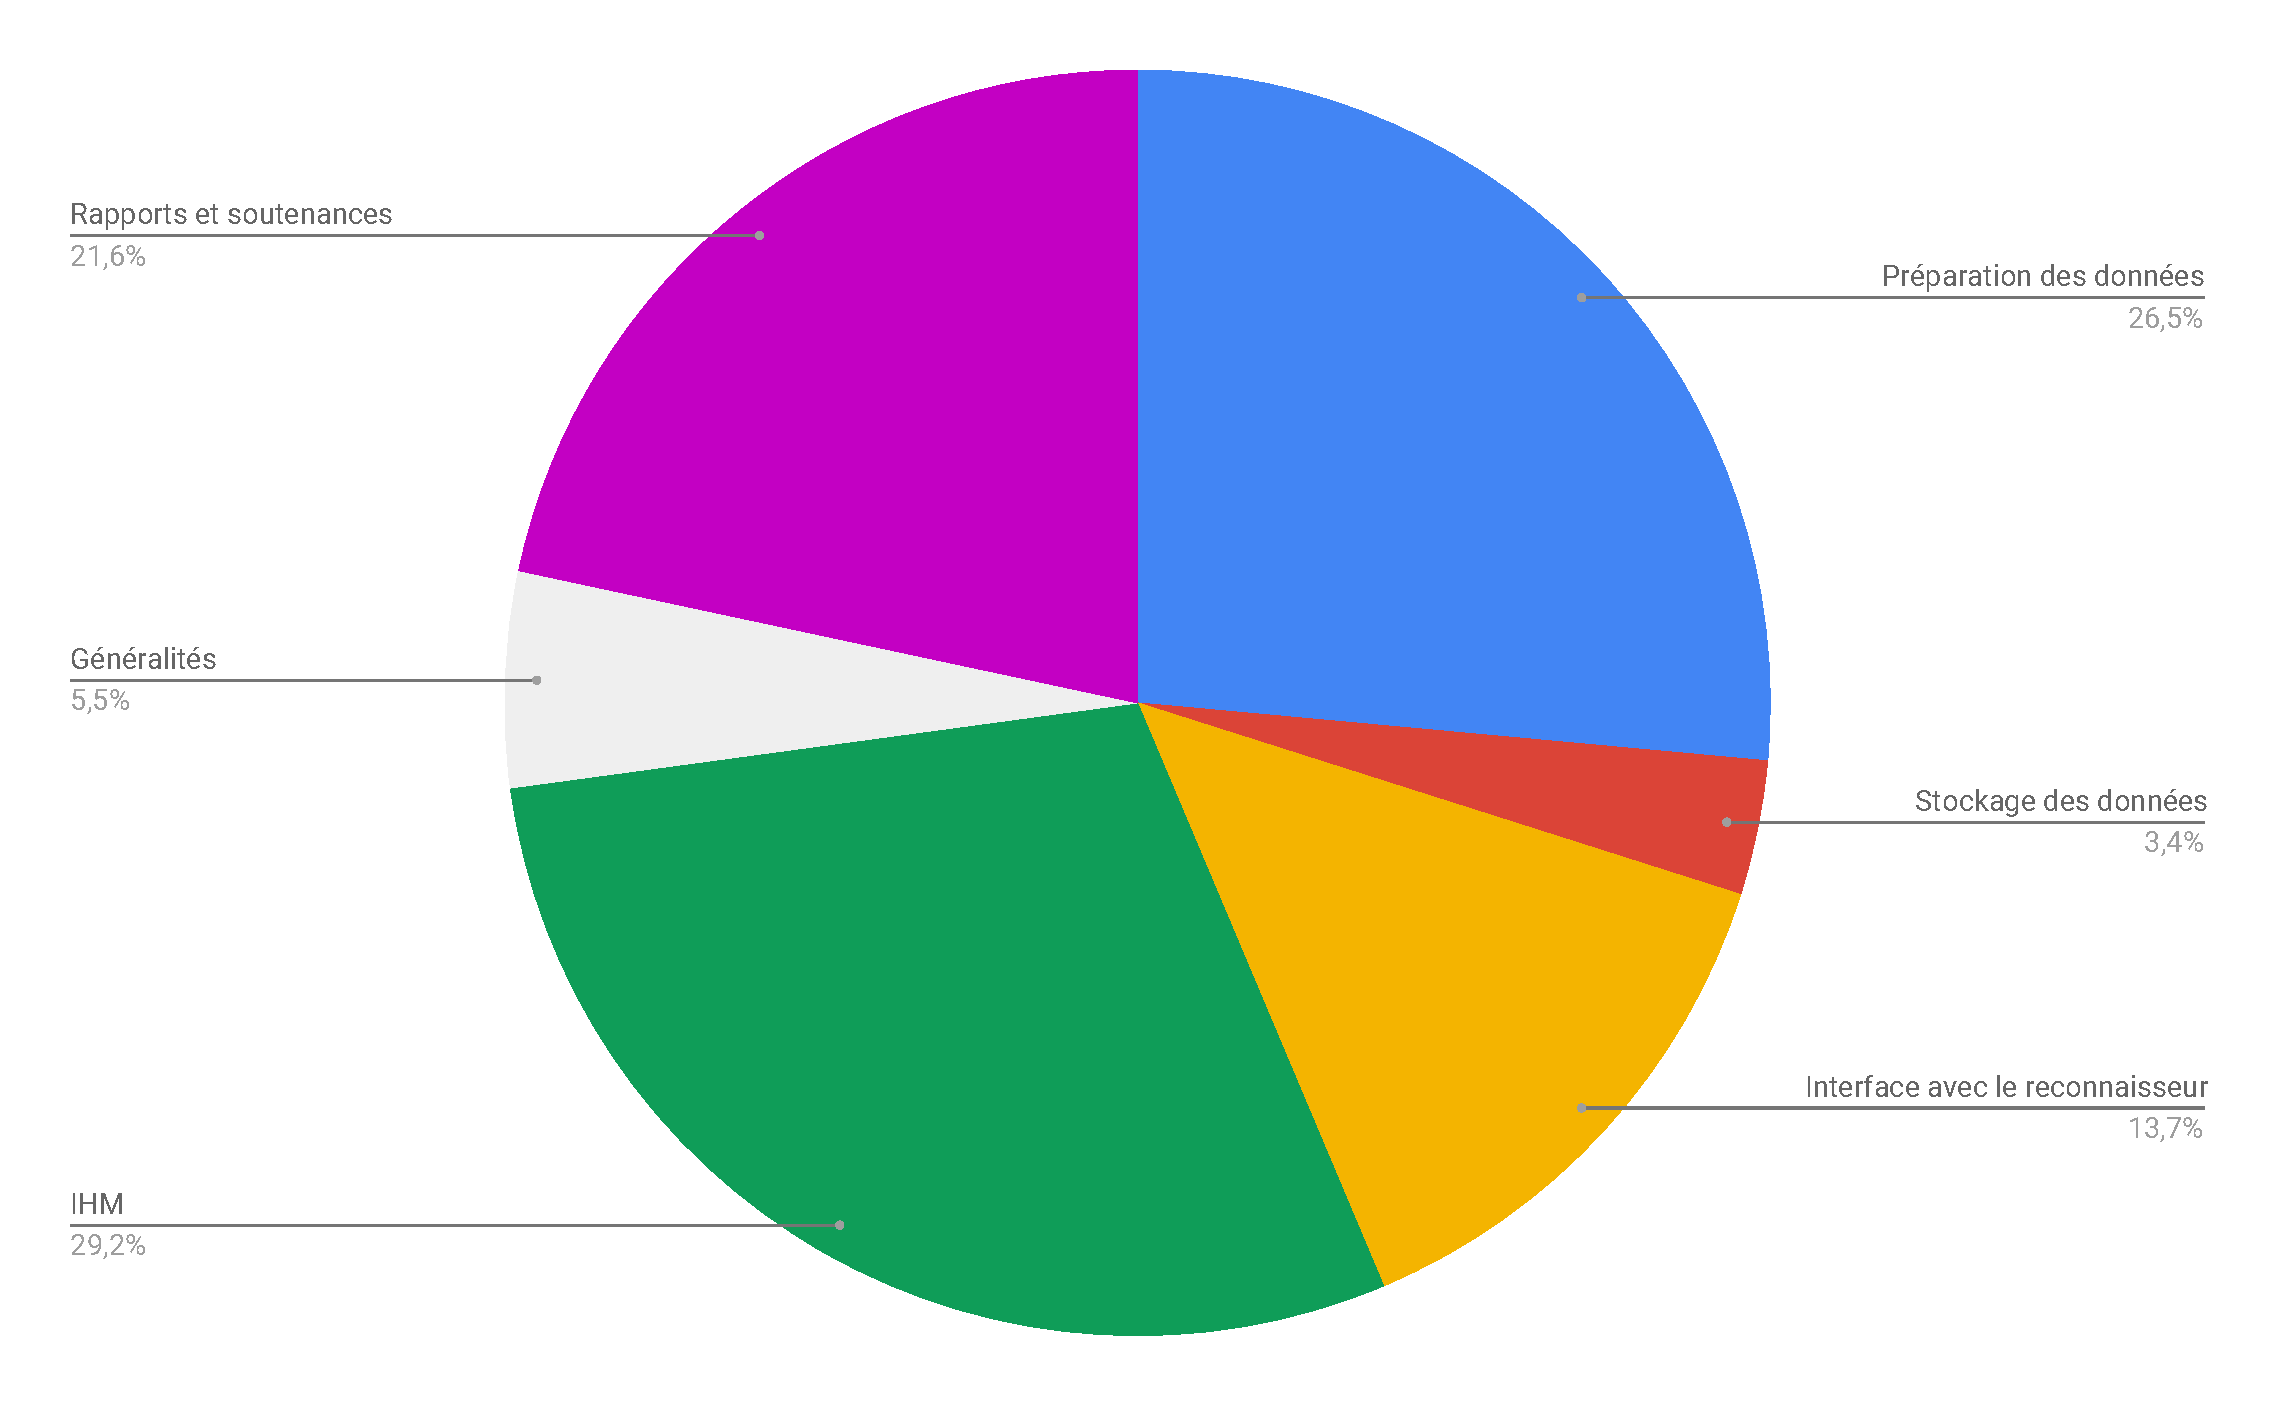
\includegraphics[scale=0.44]{repartition_travail_blocs.pdf}
\end{center}
\end{mdframed}

\section{Affectation des ressources par tâche}

Nous avons fait le choix de spécifier une ressource générique, un membre de l’équipe dans notre cas. Ce choix nous permet de garder une certaine liberté sur l’attribution des tâches durant le développement en nous permettant notamment d’affecter les tâches à un autre développeur à un instant donné. Pour le moment les développeurs ont été répartis sur chacun des blocs mais si certains blocs avancent plus vite que d’autres, il sera possible de réattribuer les rôles. Nous avons essayé de mettre au moins deux personnes par tâche pour que personne ne se retrouve seul face à un problème. Pour les tâches plus simples ou plus rapides nous n'avons mis qu'une seule personne.

\paragraph{}

Ainsi Laure et Charlotte travaillent sur la partie IHM, cette partie étant importante et comprenant suffisamment de travail pour nécessiter deux personnes dessus s’y consacrant entièrement. Timothée travaille sur la partie interface avec le reconnaisseur, cette partie est plus petite que les autres et ne nécessite qu’une personne pour être réalisée. 

\paragraph{}

La partie stockage des données est une partie différente des autres car la base de données a déjà été terminée lors du premier semestre. Ainsi, Timothée et Valentin travailleront dessus au début du second semestre pour vérifier son bon fonctionnement puis Valentin travaillera dessus seul pour terminer l’interface permettant d’y accéder. De même, le développement de la partie préparation des données a été entamé durant le premier semestre. Bien qu’étant une partie importante du projet, elle est déjà bien avancée. De fait, au début du second semestre, Enzo travaillera seul dessus, puis il sera rejoint par Valentin pour l’aider.

\paragraph{}

Concernant la répartition du travail sur les rapports, il a été estimé un travail égal pour chaque personne. Etant donné que les membres de l’équipe sont répartis en blocs, au moins un membre de chaque doit écrire une partie du rapport. Nous sommes donc partis du principe que le travail sur le rapport serait équitablement réparti dans chaque bloc, mais la répartition intra-blocs se fera en réalité au moment de l’écriture entre les membres de l’équipe.

\paragraph{}

Cette répartition permet de répartir la charge de travail de manière équilibrée. Selon notre estimation du temps de travail pour chaque tâche, chaque membre du groupe a une charge de travail égale (entre 42 et 43 heures).

\section{Jalons}

En plus de la planification du temps de développement, nous avons intégré à notre planning des jalons qui correspondent aux dates de rendus et de soutenance. Nous avons attribué l’ensemble des ressources sur les phases de préparation des rendus et des soutenances.

\section{Diagramme de Gantt}

\begin{mdframed}[frametitle={Figure 3 : Diagramme de Gantt du projet (1/2)}, innerbottommargin=10]
\begin{center}
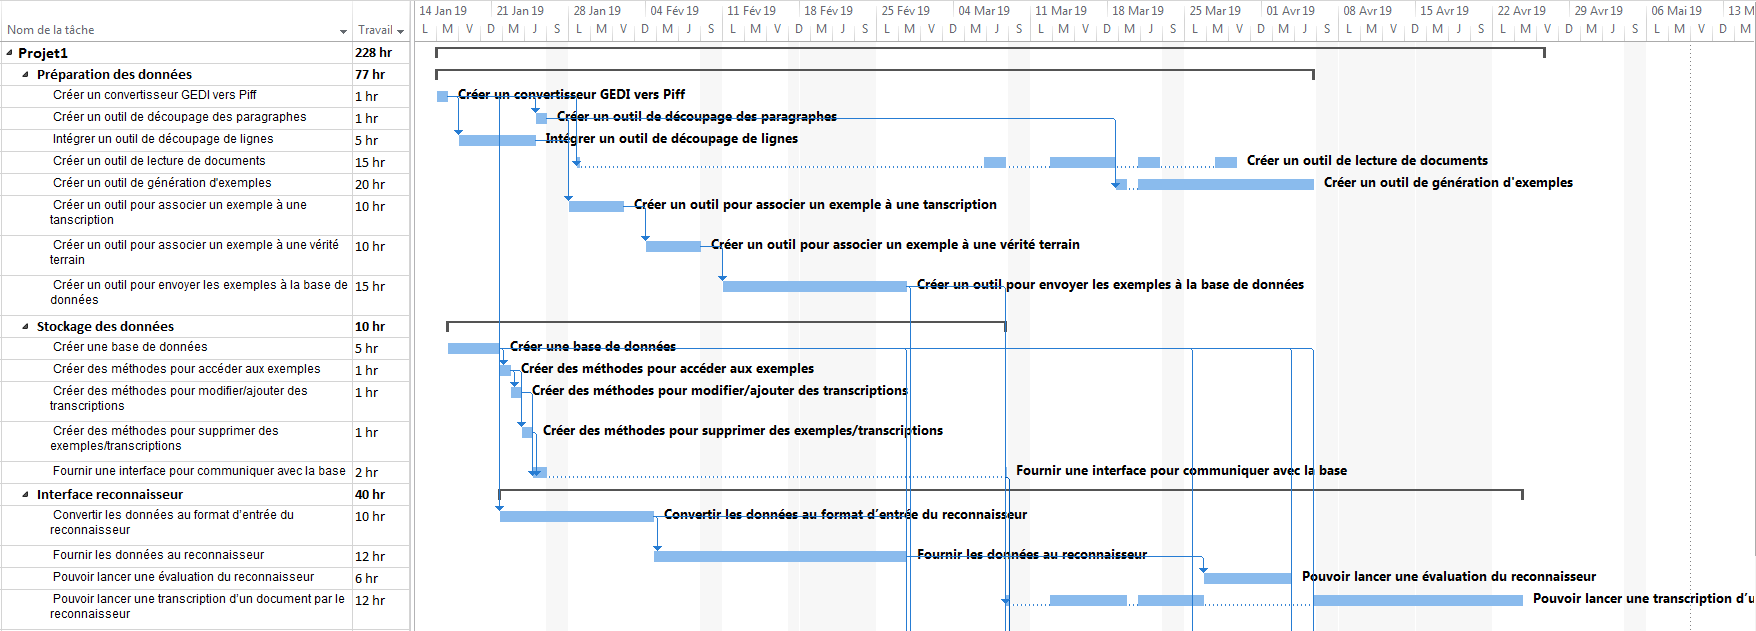
\includegraphics[scale=0.35]{gantt_V2.1.PNG}
\end{center}
\end{mdframed}

\begin{mdframed}[frametitle={Figure 4 : Diagramme de Gantt du projet (2/2)}, innerbottommargin=10]
\begin{center}
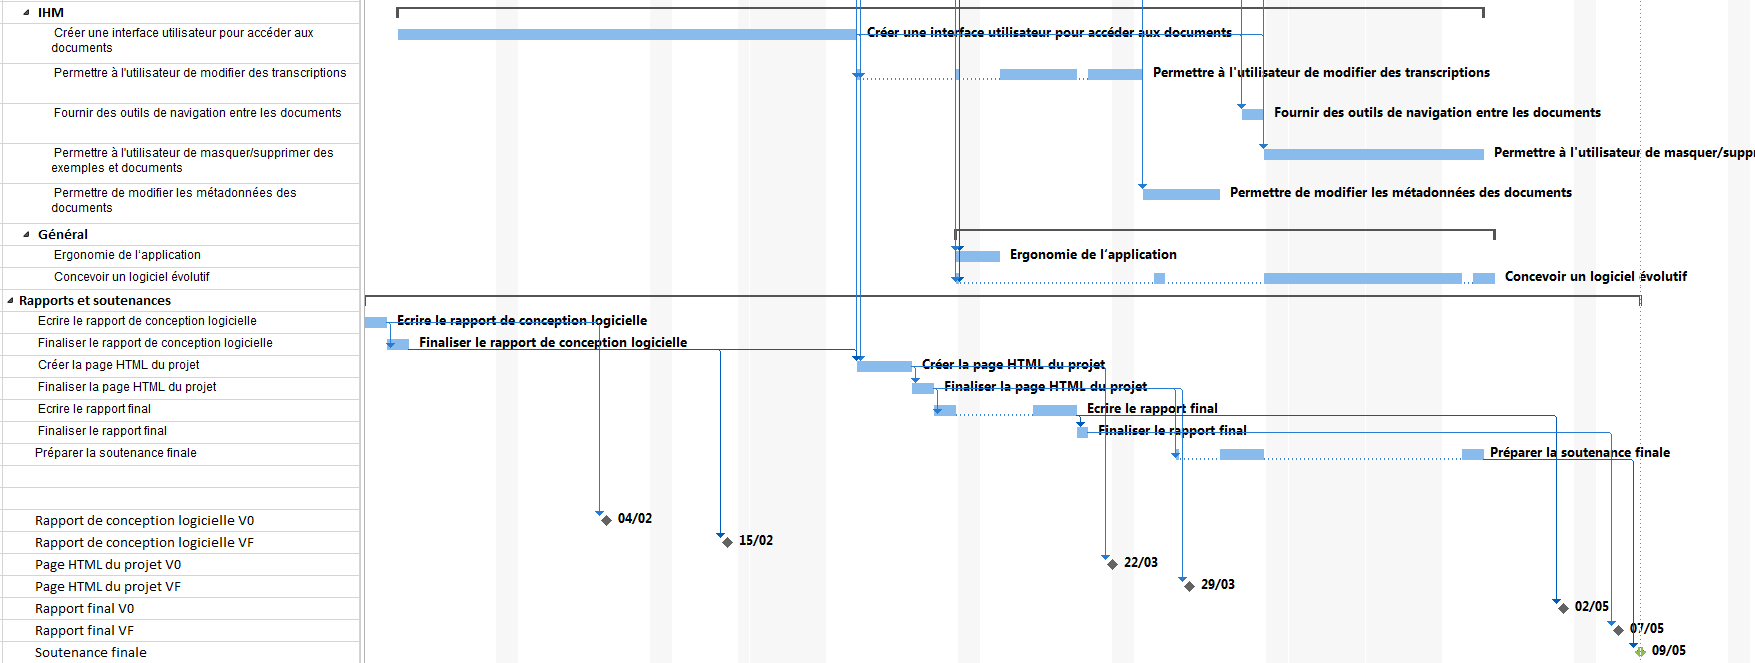
\includegraphics[scale=0.35]{gantt_V2.2.PNG}
\end{center}
\end{mdframed}

Le diagramme de Gantt ci-dessus décrit l’ensemble de la planification du projet, de la conception au rendu final en passant par la gestion de projet ou le développement de chaque itération. On y retrouve également les jalons dont nous avons parlé précédemment.

\newpage

\section{Analyse de la planification}

\subsection{Analyse globale}

Comme dit précédemment, notre projet est constitué de deux itérations. La première itération est constitué des tâches à effectuer avant la création de la page HTML. La seconde est composée des tâches restantes. Comme on peut le voir sur le diagramme, les quatre blocs sont biens parallèles et découpés en tâches. On peut constater que les tâches sont réparties uniformément entre les différents blocs mais que la partie IHM se termine après les autres. Cette partie étant en effet, plus volumineuse, les membres du groupe qui auront terminé leur partie pourront éventuellement aller aider à développer l’IHM en fin  de projet.

\subsection{Tâches critiques}

A partir du diagramme de Gantt, on peut voir apparaître deux tâches critiques, bloquant l’avancement du projet.

\begin{itemize}
\item la création d’un convertisseur GEDI vers Piff est une tâche nécessaire pour l’ensemble des tâches de la préparation de données et de l’interface avec le reconnaisseur ;
\item la création de la base de données est une étape nécessaire pour intégrer la majorité des fonctionnalités de l’IHM .
\end{itemize}

\paragraph{}

Ces tâches doivent être effectuées en priorité pour que le projet puisse avancer. Elles influent en effet sur plusieurs parties du projet. Une fois ces tâches effectuées, la majorité du projet peut se paralléliser. Cet aspect critique a été déduit intuitivement lors de la phase de spécifications du projet, c‘est pourquoi leur développement a été entamé au premier semestre. L’étude avec Microsoft Project a permis de confirmer l’aspect impératif de ces tâches.

\subsection{Ce que l'on peut retenir}

Grâce au diagramme de Gantt, nous avons pu estimer l’organisation de notre travail au second semestre. Selon cette estimation, la date de fin de projet est fixée au vendredi 26 avril. Ce qui nous laisse deux semaines d’avance, avant le dernier rendu. Nous avons également pu confirmer que l’ensemble de notre projet est faisable dans le temps qui nous est imparti. De même, selon Microsoft Project, la réalisation de la première itération pourra être réalisée pour le 27 février. Nous disposerons alors d’une première réalisation fonctionnelle de notre projet, nous aurons du temps pour améliorer cette première version, en collaboration avec le client.














